\chapter{Практическая часть}\label{ux43fux440ux430ux43aux442ux438ux447ux435ux441ux43aux430ux44f-ux447ux430ux441ux442ux44c}

\section{Цели, задачи и методология практического исследования}\label{ux446ux435ux43bux438-ux437ux430ux434ux430ux447ux438-ux438-ux43cux435ux442ux43eux434ux43eux43bux43eux433ux438ux44f-ux43fux440ux430ux43aux442ux438ux447ux435ux441ux43aux43eux433ux43e-ux438ux441ux441ux43bux435ux434ux43eux432ux430ux43dux438ux44f}

Основной целью практической части данной работы является разработка и исследование программного средства для автоматической генерации названий растений и продуктов питания на основе методов машинного обучения, а также эмпирическая проверка качества полученных моделей. Теоретические положения, изложенные в первой главе, задают общие принципы построения генеративных моделей, однако их применение к конкретной предметной области требует решения целого комплекса инженерных и методологических задач. Абстрактные рассуждения о преимуществах LSTM и трансформеров необходимо перевести в плоскость практической реализации: выбрать архитектуру, подготовить данные, настроить гиперпараметры и объективно измерить результат.

Для достижения поставленной цели были сформулированы и последовательно решены следующие задачи:

Формирование предметной области и списка категорий. Прежде чем приступать к сбору данных, необходимо было определить, какие именно названия будет генерировать система. В качестве предметной области выбраны растения (сельскохозяйственные культуры) и продукты питания. Внутри каждого направления выделены пять категорий, отражающих ключевые подобласти: для растений -- зерновые, овощные, плодовые, травы и ягоды; для продуктов -- молочные, мясные, хлебобулочные, напитки и зерновые продукты. Такое деление позволяет пользователю выбирать не просто «растение» или «продукт», а конкретный тип названия, что делает генерацию более осмысленной.

Сбор и подготовка датасета. На основе открытых источников, справочников и собственных дополнений был сформирован исходный корпус названий. Каждое название отнесено к одной из пяти категорий и размечено по количеству слов (одно, два или три). Проведена очистка данных: удалены дубликаты, исправлены опечатки, приведены к единому регистру. Подготовленный датасет послужил основой для обучения всех последующих моделей.

Аугментация данных. Поскольку исходный корпус оказался сравнительно небольшим (несколько сотен названий на категорию), была применена процедура аугментации -- искусственного расширения датасета за счёт комбинаторики. Для каждого названия, состоящего из одного слова (например, «Пшеница»), были сгенерированы дополнительные варианты путём добавления прилагательных («Пшеница Золотая», «Пшеница Северная» и так далее). Это позволило существенно увеличить объём обучающих данных и улучшить качество генерации.

Реализация генеративной LSTM-модели. На языке Python с использованием библиотеки PyTorch была реализована посимвольная LSTM-модель, генерирующая названия по заданной категории и длине. Модель обучена на подготовленном датасете, для неё подобраны гиперпараметры (размер скрытого состояния, количество слоёв, скорость обучения), проведён контроль переобучения с помощью валидационной выборки и ранней остановки.

Реализация моделей скоринга. Для оценки качества сгенерированных названий реализованы три дополнительные модели: классификатор стилей на основе свёрточной нейронной сети (char-CNN), оценщик правдоподобности на основе биграммной языковой модели и оценщик новизны на основе n-граммного сравнения. Эти модели используются для ранжирования сгенерированных названий, чтобы пользователь видел в первую очередь наиболее качественные варианты.

Разработка пользовательского интерфейса. Создано настольное приложение на базе библиотеки Gradio, предоставляющее удобный интерфейс для генерации названий. Приложение содержит две вкладки -- «Растения» и «Продукты», -- в каждой из которых пользователь может выбрать категорию, длину названия, количество результатов и при желании задать seed для воспроизводимости. Реализованы функции копирования, добавления в избранное и экспорта в текстовый файл.

Проведение экспериментального исследования. Обученные модели протестированы на отложенной выборке, измерены метрики качества: перплексия, точность классификатора стилей, доля новых названий, разнообразие. Проведено сравнение с базовыми моделями (марковская цепь, n-граммы с методом Кнесера -- Нея), а также субъективная оценка сгенерированных названий несколькими независимыми респондентами.

Методология исследования базируется на принципах эмпирического анализа алгоритмов машинного обучения. В качестве основного инструмента выбраны язык программирования Python и библиотека PyTorch. Этот выбор обусловлен рядом причин. Во-первых, PyTorch обладает интуитивно понятным API и позволяет сосредоточиться на логике модели, а не на низкоуровневых деталях. Во-вторых, он хорошо документирован и широко используется как в образовательных, так и в производственных проектах. В-третьих, он обеспечивает достаточную производительность на центральном процессоре, что критически важно для локального приложения, не требующего графического ускорителя.

Работа выполнялась поэтапно. На первом этапе были собраны и подготовлены исходные данные, сформирован корпус названий. На втором этапе проведена аугментация данных и разделение на обучающую, валидационную и тестовую выборки. На третьем этапе реализованы и обучены модели (LSTM-генератор, классификатор стилей, оценщики правдоподобности и новизны). На четвёртом этапе разработан пользовательский интерфейс и реализован пайплайн генерации, объединяющий все модели в единую систему. Наконец, на пятом, аналитическом, этапе проведены замеры качества, сравнение с бейзлайнами и интерпретация результатов.

Важно подчеркнуть, что все этапы выполнялись в рамках единого проекта, оформленного в виде репозитория на GitHub. Каждый модуль снабжён тестами, что обеспечивает воспроизводимость и надёжность результатов. Такой системный подход позволяет гарантировать достоверность полученных выводов и их практическую значимость.

\section{Сбор и подготовка датасета названий}\label{ux441ux431ux43eux440-ux438-ux43fux43eux434ux433ux43eux442ux43eux432ux43aux430-ux434ux430ux442ux430ux441ux435ux442ux430-ux43dux430ux437ux432ux430ux43dux438ux439}

Качество модели зависит от полноты и корректности обучающих данных. Для данной задачи корпус должен охватывать категории растений и продуктов, не содержать опечаток и повторов и отражать типичные структуры названий.

Для растений использовались справочники сельскохозяйственных культур, энциклопедические статьи и базы данных. Для продуктов применялись справочники, кулинарные энциклопедии, ГОСТы и технические регламенты; часть записей добавлена вручную.

Собранные названия были распределены по десяти категориям: пяти для растений и пяти для продуктов. Внутри каждой категории названия дополнительно размечались по количеству слов: одно слово (родовое название, например, «Пшеница»), два слова (родовое название с прилагательным, например, «Пшеница Озимая») и три слова (родовое название с двумя прилагательными, например, «Пшеница Озимая Твёрдая»). Такая разметка позволяет модели генерировать названия заданной длины -- от одного до трёх слов.

Исходный корпус включал около пятисот названий растений и пятисот названий продуктов -- примерно по 90--100 примеров на категорию. Этого достаточно для начального обучения компактной модели, но для повышения устойчивости далее применялась аугментация.

Предобработка данных. После сбора исходного корпуса была проведена тщательная предобработка, включающая несколько этапов.

Сначала все записи приведены к единому регистру: первая буква каждого слова стала заглавной, остальные -- строчными. Это устраняет различия, возникающие при объединении данных из разных источников.

Затем оставлены только кириллица, дефис, апостроф и пробел; случайные цифры, латинские буквы и служебные символы удалены.

Записи короче трёх символов без учёта пробелов исключены как неинформативные. Верхняя граница длины не задавалась, поскольку в корпусе есть многословные названия.

Повторы удалялись без учёта регистра: одинаковые названия, полученные из разных источников, оставлялись в одном экземпляре.

Завершающим этапом стала ручная проверка: исправлены опечатки и удалены записи, не являющиеся названиями.

\textbf{Листинг 2.2.1 -- Фрагмент функции нормализации названий}

\lstinputlisting{code/listing_01.py}

Формат хранения. Подготовленный датасет сохранён в формате JSON. Каждая запись представляет собой объект с четырьмя полями: название, категория (например, «cereal» для зерновых), источник (метка, указывающая, откуда взято название) и количество слов. Такой формат удобен как для машинной обработки, так и для ручного просмотра и редактирования. При необходимости пользователь может легко добавить новые названия, дописав их в JSON-файл и перезапустив обучение.

Разделение на выборки. Для обучения и оценки моделей датасет был разделён на три части: обучающую (80\% данных), валидационную (10\%) и тестовую (10\%). Разделение проводилось стратифицированно -- с сохранением пропорций категорий в каждой выборке. Это гарантирует, что модель обучается на всех категориях одновременно и проверяется на примерах из всех категорий. Дополнительно проверялось отсутствие утечки данных: ни одно название из обучающей выборки не должно встречаться в валидационной или тестовой.

Итоговые характеристики. После предобработки исходный датасет содержал 499 названий растений и 498 названий продуктов, распределённых по пяти категориям каждое. По количеству слов распределение оказалось следующим: около 20\% -- односложные названия, около 30\% -- двухсловные, около 50\% -- трёхсловные. Такое распределение отражает реальную практику: в сельском хозяйстве и пищевой промышленности большинство названий включают уточняющие прилагательные, поэтому трёхсловные названия встречаются часто.

Подготовленный датасет стал отправной точкой для всех последующих этапов. На его основе проводилась аугментация (раздел 2.3), обучение моделей (раздел 2.4) и оценка качества. Важно отметить, что качество датасета напрямую влияет на качество генерации: чем больше разнообразных и корректных примеров видит модель, тем лучше она учится и тем более осмысленные названия порождает.

\section{Аугментация данных и разметка по категориям}\label{ux430ux443ux433ux43cux435ux43dux442ux430ux446ux438ux44f-ux434ux430ux43dux43dux44bux445-ux438-ux440ux430ux437ux43cux435ux442ux43aux430-ux43fux43e-ux43aux430ux442ux435ux433ux43eux440ux438ux44fux43c}

Как было отмечено в предыдущем разделе, исходный датасет содержал около тысячи названий -- по 500 для растений и продуктов. Для обучения LSTM-модели этого объёма недостаточно: модель склонна к переобучению, генерирует однообразные названия и плохо справляется с длинными конструкциями. В данном разделе описано, как была проведена аугментация данных -- искусственное расширение корпуса за счёт комбинаторики.

Идея аугментации. В исходном датасете многие названия имеют структуру «существительное + прилагательное» (например, «Пшеница Золотая») или «существительное + прилагательное + прилагательное» (например, «Пшеница Золотая Скороспелая»). При этом количество возможных комбинаций существенно превышает число примеров в датасете. Например, если в корпусе есть десять родовых названий (Пшеница, Рожь, Ячмень, Овёс, Кукуруза, Рис, Просо, Гречиха, Сорго, Тритикале) и десять прилагательных женского рода (Золотая, Северная, Южная, Ранняя, Поздняя, Крупная, Мелкая, Скороспелая, Урожайная, Отборная), то только для двухсловных названий можно составить сто комбинаций. В датасете же присутствует лишь часть из них.

Аугментация заключается в том, чтобы искусственно достроить отсутствующие комбинации. Это не «фейковые данные»: все новые названия грамматически корректны и семантически осмысленны. Модель, обучаясь на расширенном корпусе, видит гораздо больше примеров и лучше усваивает закономерности. В результате она генерирует более разнообразные и правильные названия.

Механизм аугментации. Процедура аугментации реализована в отдельном скрипте, который выполняется после сбора и предобработки данных. Работа скрипта состоит из следующих шагов.

На первом шаге для каждой категории собираются все существительные (родовые названия), встречающиеся в однословных названиях, и все прилагательные, встречающиеся в двухсловных названиях. Существительные группируются по роду: женский, мужской, средний и множественное число. Прилагательные также группируются по роду. Это необходимо для того, чтобы при комбинировании не возникало грамматических ошибок («Пшеница Золотой» вместо «Пшеница Золотая»).

На втором шаге для каждого существительного подбираются прилагательные того же рода и формируются новые двухсловные названия. Например, для существительного «Пшеница» (женский род) берутся прилагательные женского рода и составляются пары: «Пшеница Золотая», «Пшеница Северная», «Пшеница Скороспелая» и так далее. Процесс повторяется для всех существительных и всех прилагательных.

На третьем шаге аналогичным образом формируются трёхсловные названия: для каждого существительного выбираются два прилагательных того же рода, и составляется название из трёх слов. Например, «Пшеница Золотая Скороспелая», «Рожь Северная Урожайная» и так далее.

На четвёртом шаге проводится проверка на дубликаты: если сгенерированное название уже присутствует в датасете (например, оно было в исходном корпусе), оно пропускается. Это гарантирует, что аугментация только добавляет новые записи и не создаёт повторов.

Учёт рода существительных. Отдельного внимания заслуживает проблема определения рода. В русском языке род существительного не всегда можно однозначно определить по окончанию. Например, слово «Рожь» оканчивается на мягкий знак, и без словаря невозможно сказать, мужского оно рода или женского (на самом деле -- женского). Если бы мы определяли род только по окончанию, то для «Ржи» подобрали бы прилагательные мужского рода и получили бы грамматически неверное «Рожь Золотой».

Для решения этой проблемы был создан явный словарь родов -- таблица, в которой для каждого существительного указан его род. Словарь охватывает все существительные, встречающиеся в датасете, и включает как женский и мужской род, так и средний, а также множественное число. При аугментации программа обращается к этому словарю, а не к эвристике по окончанию. Это гарантирует грамматическую корректность всех сгенерированных названий.

Отдельно стоит упомянуть слова во множественном числе -- например, «Отруби», «Хлебцы», «Крекеры», «Сушки». Эти существительные требуют прилагательных во множественном числе: «Отруби Питательные», «Хлебцы Пшеничные», «Сушки Цельнозерновые». В словаре родов для них предусмотрена специальная категория «множественное число», а в списке прилагательных -- соответствующие формы множественного числа.

Расширение списка прилагательных. Помимо комбинирования существующих прилагательных, был составлен дополнительный список прилагательных, характерных для растений и продуктов. Этот список включает как универсальные прилагательные («Золотая», «Крупная», «Отборная»), так и специфичные для конкретных категорий («Озимая», «Яровая», «Скороспелая» для зерновых; «Столовая», «Салатная», «Засолочная» для овощей; «Садовая», «Лесная», «Ремонтантная» для ягод). Каждое прилагательное представлено в трёх родах и, где необходимо, во множественном числе.

Результаты аугментации. После применения аугментации объём датасета вырос примерно в три раза. Для растений из 499 исходных названий получилось около 1500, для продуктов -- аналогично. Распределение по количеству слов сместилось в сторону двух- и трёхсловных названий, что соответствует реальной практике: в сельском хозяйстве и пищевой промышленности большинство названий включают уточняющие прилагательные.

Разметка по категориям. Помимо разметки по количеству слов, каждое название размечено по категории. Категории для растений: «cereal» (зерновые), «vegetable» (овощные), «fruit» (плодовые), «herb» (травы), «berry» (ягоды). Для продуктов: «dairy» (молочные), «meat» (мясные), «bakery» (хлебобулочные), «drink» (напитки), «grain» (зерновые продукты). Разметка по категориям необходима для обучения классификатора стилей и для условной генерации: модель должна генерировать названия именно той категории, которую выбрал пользователь.

Разметка проводилась вручную на этапе сбора данных. Каждое название было отнесено к одной из пяти категорий на основе его значения. В дальнейшем эта разметка использовалась при обучении классификатора и при оценке качества генерации.

Итоговые характеристики. После аугментации датасет содержал около 1500 названий растений и 1500 названий продуктов, распределённых по пяти категориям каждое. Средняя длина названия составила 2--3 слова, что соответствует реальным названиям в аграрной сфере. Такой объём является достаточным для обучения LSTM-модели среднего размера, не перегруженной параметрами, и позволяет достичь стабильного качества генерации.

\section{Архитектура генеративной модели на основе LSTM}\label{ux430ux440ux445ux438ux442ux435ux43aux442ux443ux440ux430-ux433ux435ux43dux435ux440ux430ux442ux438ux432ux43dux43eux439-ux43cux43eux434ux435ux43bux438-ux43dux430-ux43eux441ux43dux43eux432ux435-lstm}

Центральным элементом разработанной системы является генеративная модель на основе рекуррентной нейронной сети с долгой краткосрочной памятью (LSTM). Именно она отвечает за порождение новых названий растений и продуктов. В данном разделе описано, как устроена эта модель, какие архитектурные решения были приняты и как проходил процесс обучения.

Общая схема работы. Модель работает посимвольно: она получает на вход последовательность символов и предсказывает следующий символ. Процесс генерации начинается со специального маркера начала и продолжается до тех пор, пока модель не выдаст маркер конца или не будет достигнута максимальная длина названия. Каждый предсказанный символ добавляется к последовательности и подаётся на вход на следующем шаге. В результате модель порождает название целиком -- от первого символа до последнего.

Дополнительные условия. Для того чтобы пользователь мог управлять генерацией, модель получает не только последовательность символов, но и два дополнительных условия: категорию (например, «cereal» для зерновых) и количество слов в названии (одно, два или три). Эти условия подаются в модель в виде векторных представлений (эмбеддингов) и конкатенируются с символьными представлениями на каждом шаге. Благодаря этому модель учится генерировать разные названия для разных условий: зерновые названия будут отличаться от ягодных, а двухсловные -- от трёхсловных.

Категории кодируются как целые числа от 0 до 4 (для пяти категорий каждого домена). Количество слов кодируется как 1, 2 или 3. Для каждого из этих значений модель имеет собственный обучаемый вектор -- эмбеддинг категории размером 32 и эмбеддинг количества слов размером 16. Эти размеры были подобраны экспериментально: они достаточно велики, чтобы вмещать смысловую информацию о категории и длине, но при этом не создают избыточного числа параметров.

Символьные эмбеддинги. Каждый символ из словаря (включая маркеры начала, конца и паддинга) получает собственное векторное представление размером 64. Такое представление позволяет модели улавливать сходство между символами: например, гласные могут получать близкие векторы, согласные -- другие. Эмбеддинги обучаются совместно с остальной моделью, то есть их значения подстраиваются под задачу генерации названий.

Архитектура LSTM. Основу модели составляет двухслойная LSTM с размером скрытого состояния 128. Первый слой получает на вход конкатенацию символьного эмбеддинга, эмбеддинга категории и эмбеддинга длины; второй слой получает выход первого. Между слоями применяется dropout с вероятностью 0.2 -- это стандартный метод регуляризации, помогающий предотвратить переобучение. Двухслойная архитектура выбрана как компромисс между выразительностью (один слой может не уловить сложные зависимости) и устойчивостью к переобучению (три и более слоёв на нашем объёме данных склонны к переобучению).

\textbf{Листинг 2.4.1 -- Фрагмент прямого прохода LSTM-модели}

\lstinputlisting{code/listing_02.py}

Выходной слой. Выход LSTM пропускается через dropout и подаётся на полносвязный слой, который преобразует скрытое состояние в распределение вероятностей по всем символам словаря. Размер словаря зависит от домена: для растений и продуктов он включает все символы, встречающиеся в соответствующих датасетах (обычно около 40 символов -- буквы русского алфавита, дефис, апостроф, пробел и специальные маркеры). На выходе получается вектор вероятностей, из которого тем или иным способом выбирается следующий символ.

Выбор следующего символа. Простой выбор самого вероятного символа приводит к тому, что модель всегда генерирует одно и то же название. Для получения разнообразных результатов применяются специальные методы сэмплирования.

Первый метод -- temperature (температура). Он управляет степенью «уверенности» модели: при низкой температуре модель предпочитает самые вероятные символы, при высокой -- более равномерно распределяет вероятность между всеми символами. Температура 1.0 соответствует исходному распределению; температура ниже 1.0 делает модель более «консервативной», выше 1.0 -- более «креативной». В приложении температура зафиксирована на значении 0.8, что даёт баланс между осмысленностью и разнообразием.

Второй метод -- top-k сэмплирование. Он ограничивает выбор k самыми вероятными символами, отбрасывая все остальные. Это позволяет избежать генерации маловероятных символов, которые могут испортить название. Значение k = 40 было выбрано как разумное для словаря из 40--50 символов: оно не слишком жёсткое, но и не позволяет модели «уходить в случайность».

Третий метод -- top-p (nucleus) сэмплирование. Он оставляет только те символы, суммарная вероятность которых превышает заданный порог p.~Это адаптивный метод: при высокой уверенности модели в распределении остаётся мало символов, при низкой -- много. Значение p = 0.9 было выбрано как стандартное и хорошо работающее на практике.

Все три метода применяются последовательно: сначала temperature, затем top-k, затем top-p, и только после этого из оставшегося распределения случайно выбирается символ.

Процесс обучения. Обучение модели проводилось на подготовленном датасете (около 1500 названий на домен). Датасет разделён на обучающую (80\%), валидационную (10\%) и тестовую (10\%) выборки. Обучение длилось до 200 эпох с ранней остановкой: если в течение 25 эпох валидационная ошибка не улучшалась, обучение прекращалось. Это позволило избежать переобучения и сэкономить время.

В качестве функции потерь использовалась кросс-энтропия -- стандартная функция для задач классификации, к которым относится и предсказание следующего символа. Оптимизатор -- Adam с начальной скоростью обучения 1e-3 и weight decay 1e-5 (лёгкая L2-регуляризация). Размер батча -- 16. Все эти значения были подобраны экспериментально и показали стабильные результаты.

Обучение одной модели занимает около одной-двух минут на центральном процессоре. Это позволяет быстро переобучать модель при изменении датасета -- что важно для практического использования.

Результаты обучения. После обучения LSTM-модель для растений показала перплексию около 4--5 на валидационной выборке, для продуктов -- аналогично. Это означает, что модель достаточно уверенно предсказывает следующий символ и хорошо улавливает закономерности в названиях. Сгенерированные названия в большинстве случаев звучат правдоподобно и соответствуют заданной категории.

Сохранение и загрузка модели. Обученная модель сохраняется в файл формата .pt (формат библиотеки PyTorch). Файл содержит веса модели, словарь символов и конфигурацию архитектуры. При запуске приложения модель загружается из файла один раз и используется для всех последующих генераций. Это обеспечивает высокую скорость работы: пользователь не ждёт переобучения модели при каждом запросе.

\section{Модели скоринга и ранжирования}\label{ux43cux43eux434ux435ux43bux438-ux441ux43aux43eux440ux438ux43dux433ux430-ux438-ux440ux430ux43dux436ux438ux440ux43eux432ux430ux43dux438ux44f}

Генеративная LSTM-модель порождает названия, но не все из них оказываются одинаково качественными. Некоторые названия звучат правдоподобно, другие -- неудачно, третьи -- повторяют уже существующие. Для того чтобы пользователь видел в первую очередь лучшие варианты, в системе реализован дополнительный слой -- модели скоринга и ранжирования. В данном разделе описаны три модели, входящие в этот слой: классификатор стилей, оценщик правдоподобности и оценщик новизны.

Классификатор стилей -- это нейросетевая модель, которая определяет, к какой категории относится название. Она обучена на том же датасете, что и LSTM-генератор, и решает задачу классификации на пять классов (для растений -- зерновые, овощные, плодовые, травы, ягоды; для продуктов -- молочные, мясные, хлебобулочные, напитки, зерновые продукты). Классификатор выдаёт для каждого названия вектор вероятностей по всем категориям, и вероятность правильной категории используется как оценка стилевого соответствия: чем выше эта вероятность, тем более «типичным» для категории является название.

Архитектура классификатора -- свёрточная нейронная сеть, работающая с символьными последовательностями (char-CNN). Она получает на вход последовательность символов, преобразует каждый символ в векторное представление, а затем применяет одномерную свёртку с ядром размера 3 и 64 фильтрами. Свёртка позволяет улавливать локальные паттерны -- например, характерные окончания или сочетания букв. После свёртки применяется глобальный max-pooling (выбор максимального значения по всей длине) и полносвязный слой, выдающий вероятности категорий.

\textbf{Листинг 2.5.1 -- Фрагмент классификатора стилей}

\lstinputlisting{code/listing_03.py}

Такая архитектура хорошо подходит для коротких текстов: она компактна (около 30 тысяч параметров), быстро обучается и показывает высокую точность. На тестовой выборке точность классификатора составила около 80\%, что является хорошим результатом для задачи с пятью классами и сравнительно небольшим датасетом.

Классификатор обучался тем же способом, что и LSTM: разделение на выборки, кросс-энтропия, оптимизатор Adam, ранняя остановка. Обучение занимает около тридцати секунд на центральном процессоре.

Оценщик правдоподобности -- это модель, которая определяет, насколько название «звучит как настоящее». В отличие от классификатора, она не является нейросетью, а использует классическую статистическую модель -- биграммную языковую модель. Идея проста: для каждой пары соседних символов в названии вычисляется вероятность их совместного появления, а затем эти вероятности перемножаются. Чем выше итоговая вероятность, тем более правдоподобно название.

Для оценки пар символов используется обучающая выборка: подсчитывается, сколько раз каждая пара встречается в названиях датасета. Чтобы избежать нулевых вероятностей для пар, не встречавшихся в датасете, применяется сглаживание Лапласа -- ко всем парам добавляется небольшая константа (1.0), что гарантирует, что любая пара имеет ненулевую вероятность.

Сырая вероятность (произведение вероятностей всех пар) может быть очень маленькой и неудобной для интерпретации. Поэтому она нормируется: вычисляется среднее и стандартное отклонение по обучающей выборке, и итоговая оценка получается как нормированное значение, пропущенное через сигмоиду -- функцию, преобразующую любое число в диапазон от 0 до 1. В результате оценка правдоподобности находится в диапазоне от 0 (совершенно неправдоподобно) до 1 (полностью правдоподобно).

Такая модель не требует обучения в традиционном смысле -- она просто подсчитывает статистику по датасету. Это делает её быстрой и интерпретируемой: можно посмотреть, какие именно пары символов дали высокую или низкую оценку.

Оценщик новизны -- это модель, которая определяет, насколько сгенерированное название отличается от тех, что были в обучающем датасете. Если модель просто запоминает названия из датасета и выдаёт их, это плохо: пользователю нужны новые варианты, а не копии существующих.

Оценщик новизны работает на основе n-граммного сравнения. Каждое название разбивается на набор коротких подпоследовательностей -- n-грамм. Используются биграммы (пары символов) и триграммы (тройки символов). Например, название «Пшеница» порождает биграммы «Пш», «ше», «ен», «ни», «иц», «ца» и триграммы «Пше», «шен», «ени», «ниц», «ица». Аналогичные наборы строятся для каждого названия из обучающего датасета.

Для оценки новизны вычисляется максимальное сходство между n-граммами нового названия и n-граммами каждого из названий датасета. Сходство измеряется коэффициентом Жаккара -- отношением размера пересечения к размеру объединения множеств. Итоговая новизна равна единице минус максимальное сходство: если новое название полностью совпадает с каким-то из датасета, новизна равна 0; если не имеет ни одной общей n-граммы ни с одним названием датасета -- новизна равна 1.

Такая мера позволяет уловить не только точные копии, но и «почти копии» -- названия, которые отличаются от существующих лишь одним-двумя символами. Это важно для практического использования: пользователю нужны действительно новые варианты.

Итоговый скор. Три оценки -- стилевое соответствие, правдоподобность и новизна -- объединяются в единый итоговый скор, который используется для ранжирования. По умолчанию веса следующие: 0.5 для стилевого соответствия, 0.25 для правдоподобности, 0.25 для новизны. Такое распределение отражает приоритеты: главное -- чтобы название соответствовало заданной категории; при этом важно, чтобы оно звучало правдоподобно и было новым.

Итоговый скор вычисляется как взвешенная сумма трёх оценок. Все три оценки находятся в диапазоне от 0 до 1, поэтому итоговый скор тоже находится в этом диапазоне. При ранжировании названия сортируются по убыванию итогового скора: пользователь видит в первую очередь наиболее качественные варианты.

Важно отметить, что все три оценки вычисляются для каждого сгенерированного названия, а не только для финального результата. Это позволяет из ста сгенерированных кандидатов выбрать действительно лучшие, а не просто взять первые попавшиеся.

Пайплайн генерации. Все модели объединены в единый пайплайн, который работает следующим образом. Сначала LSTM-модель генерирует сто кандидатов по заданным условиям. Затем каждый кандидат проходит фильтр: отбрасываются названия неправильной длины, дубликаты и пустые строки. Оставшиеся названия оцениваются тремя моделями скоринга, и для каждого вычисляется итоговый скор. Наконец, названия сортируются по убыванию скора, и пользователю показываются первые N лучших.

Производительность. Вся процедура -- генерация ста кандидатов, фильтрация, скоринг и ранжирование -- занимает менее секунды на обычном процессоре. Это позволяет использовать систему интерактивно: пользователь нажимает кнопку и через мгновение видит результаты.

\section{Реализация пользовательского интерфейса}\label{ux440ux435ux430ux43bux438ux437ux430ux446ux438ux44f-ux43fux43eux43bux44cux437ux43eux432ux430ux442ux435ux43bux44cux441ux43aux43eux433ux43e-ux438ux43dux442ux435ux440ux444ux435ux439ux441ux430}

Для практического использования моделей разработан интерфейс, через который пользователь задаёт параметры генерации и работает с полученными вариантами.

Для интерфейса выбрана Gradio -- Python-фреймворк, который позволяет быстро создавать локальные веб-страницы для моделей машинного обучения без отдельной разработки HTML, CSS и JavaScript.

Tkinter и PyQt требуют разработки классического оконного интерфейса, а Flask и Django -- полноценного веб-приложения. Gradio выбрана как более простой вариант с современным интерфейсом.

Приложение открывается в браузере по адресу http://127.0.0.1:7860 и содержит две вкладки -- «Растения» и «Продукты». В шапке размещены название и краткое описание приложения.

Каждая вкладка включает три панели: параметры генерации, список результатов и избранное.

\textbf{Листинг 2.6.1 -- Фрагмент построения вкладки интерфейса}

\lstinputlisting{code/listing_04.py}

В левой панели задаются категория, длина названия (одно, два или три слова), количество результатов (от 1 до 50) и seed для воспроизводимости. Для растений и продуктов предусмотрены собственные категории.

Категория выбирается из списка, длина -- переключателем, количество -- ползунком, а seed вводится в числовое поле или генерируется случайно.

После нажатия кнопки «Сгенерировать» результаты появляются в центральной панели.

Результаты представлены списком карточек с названиями и кнопкой добавления в избранное. Список отсортирован по итоговому скору.

Пользователь может скопировать название, выделив его мышкой и нажав Ctrl+C. Это стандартное поведение браузера, не требующее дополнительной реализации.

\noindent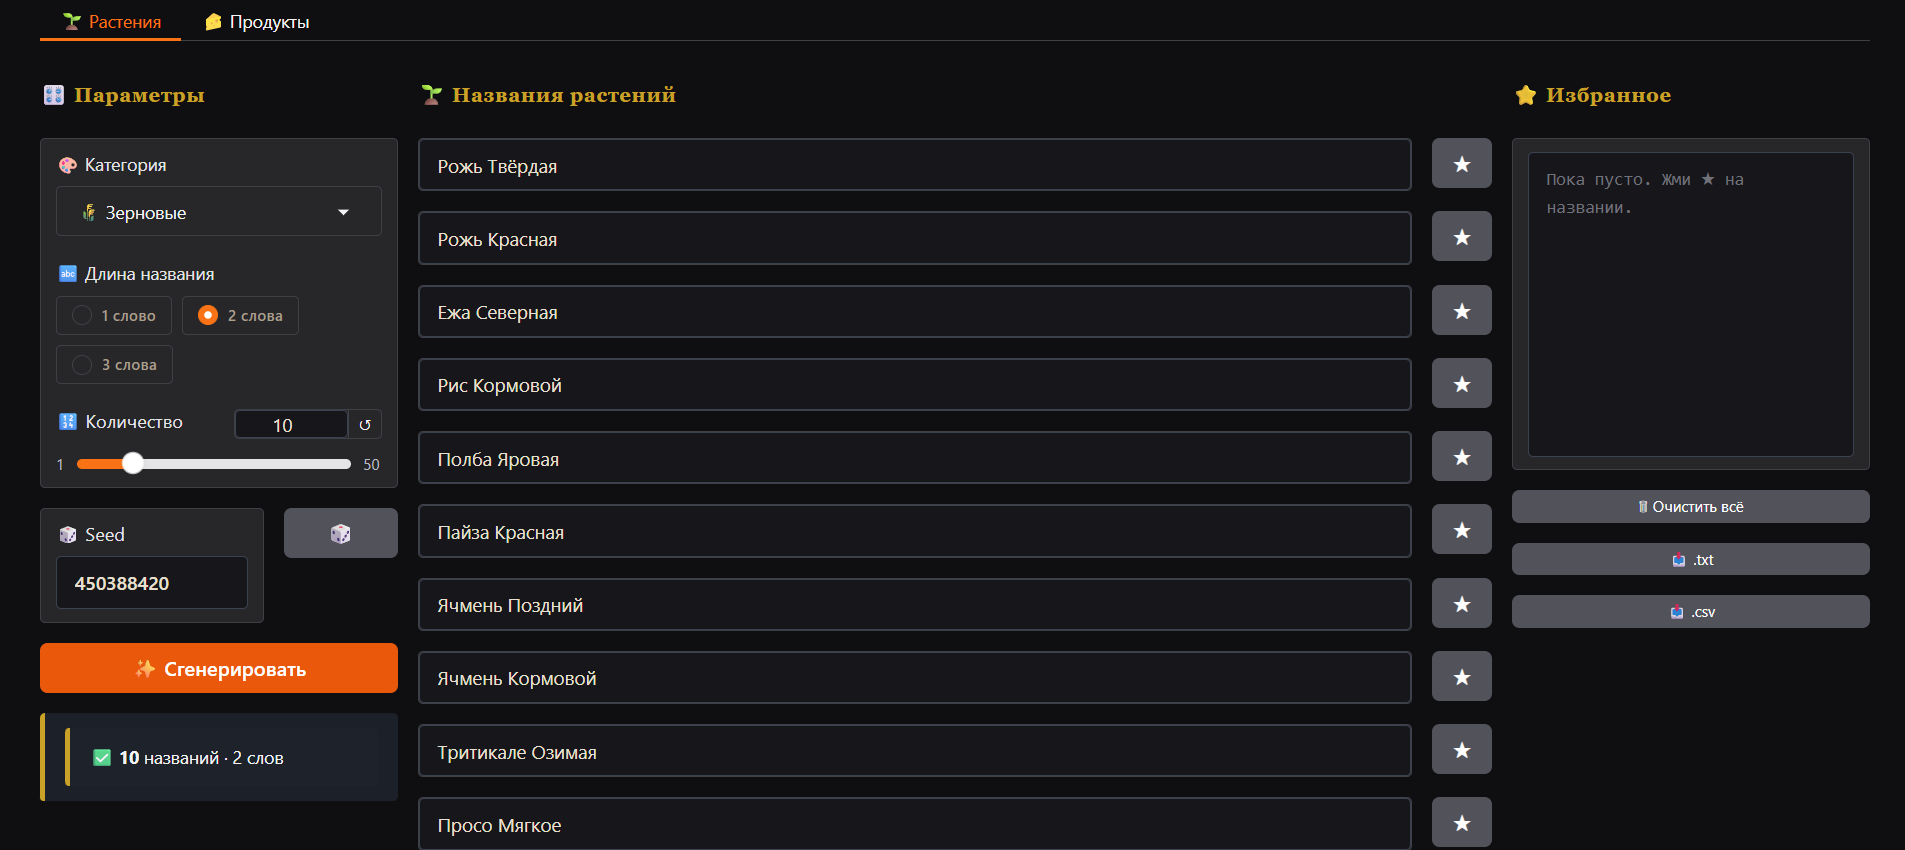
\includegraphics[width=\textwidth,keepaspectratio]{figures/image1.png}

\begin{center}\textbf{Рисунок 2.1 -- Вкладка «Растения» с результатами генерации}\end{center}

\noindent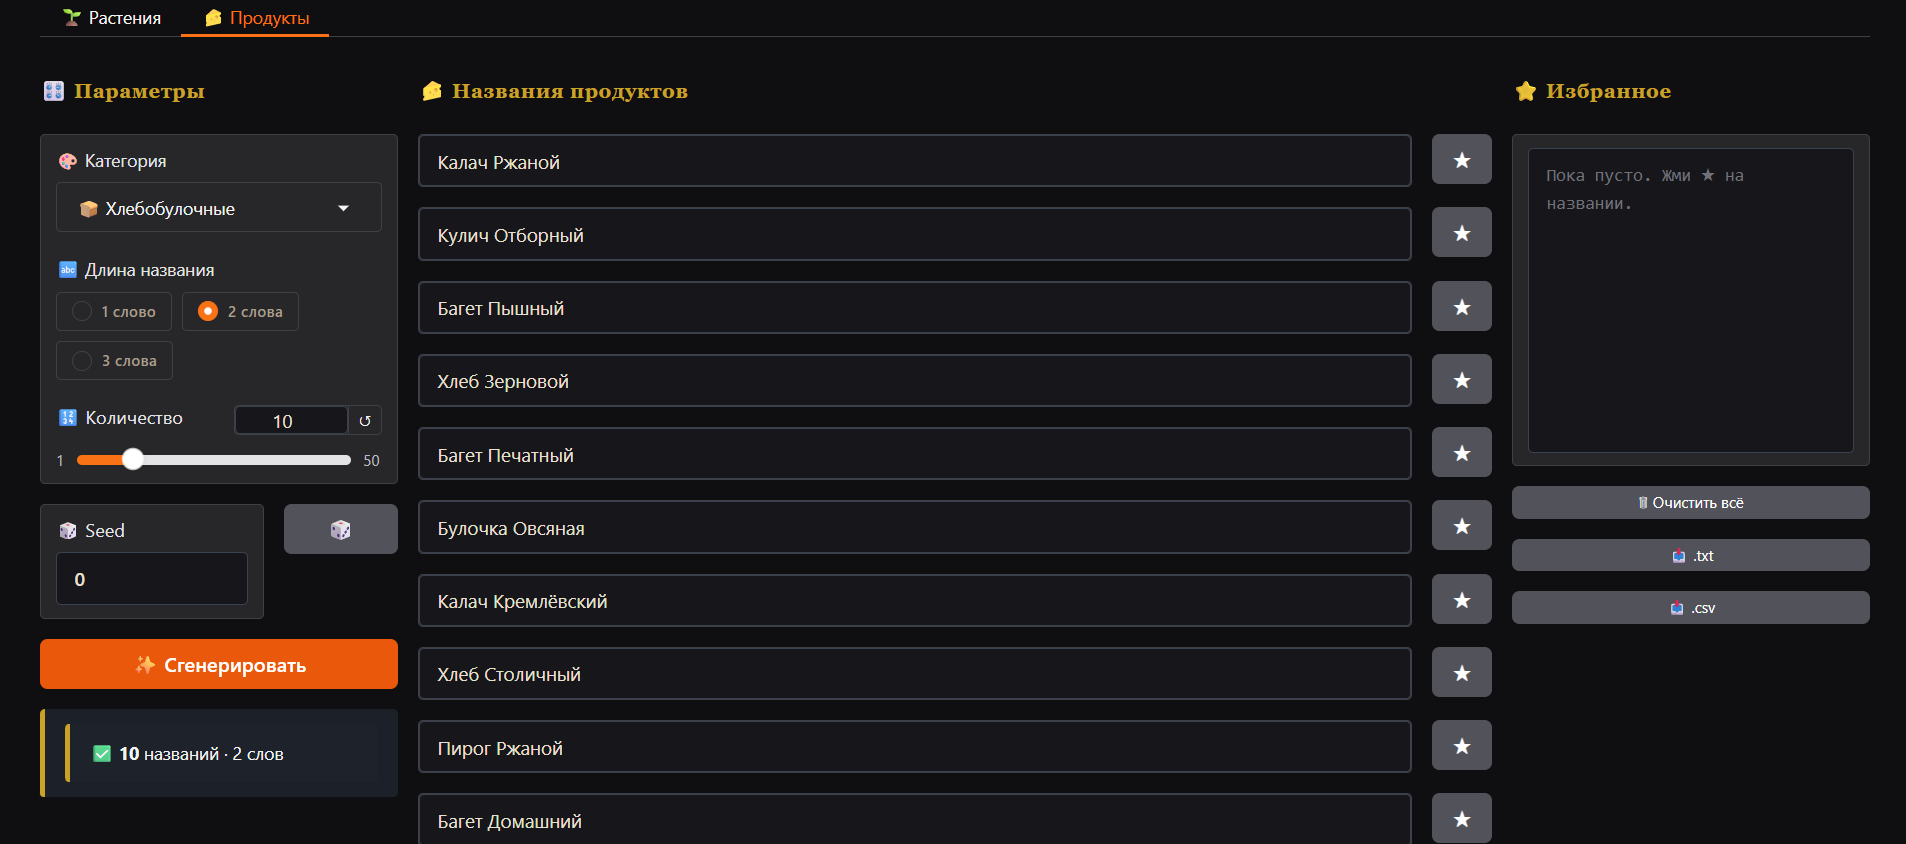
\includegraphics[width=\textwidth,keepaspectratio]{figures/image2.png}

\begin{center}\textbf{Рисунок 2.2 -- Вкладка «Продукты» с результатами генерации}\end{center}

В правой панели отображается избранное; данные растений и продуктов сохраняются отдельно. Пользователь может просматривать список, очищать его и экспортировать результаты.

Просмотреть список избранных названий.

Очистить список полностью (кнопка «Очистить всё»).

Экспортировать избранное в текстовый файл (.txt) или CSV-файл (.csv).

Файл .txt содержит по одному названию в строке, а CSV-файл -- столбец name. Оба формата подходят для дальнейшей обработки.

Избранное хранится в \path{user_data/plants_favorites.json} и \path{user_data/products_favorites.json}. Файлы создаются автоматически и сохраняются между запусками приложения.

Интерфейс оформлен в тёмной цветовой гамме с золотыми и багряными акцентами: тёмно-серый фон, контрастные панели и светлый текст.

Для распространения приложение собирается в .exe с помощью PyInstaller в режиме onedir: исполняемый файл и зависимости размещаются в одной папке. Такой вариант запускается быстрее, чем onefile, и удобен для копирования.

При первом запуске рядом с .exe создаётся папка user\_data для избранного и экспортированных файлов.

Приложение запускается за 3--5 секунд, генерация занимает менее секунды. Работа выполняется локально, без обращения к внешним сервисам.

Разработанный интерфейс объединяет основные функции системы: настройку параметров, просмотр результатов, избранное и экспорт. Приложение может использоваться локально на компьютере с Windows.
